\chapter{SeL4}
seL4 fa parte della famiglia dei microkernel L4 che risalgono alla prima metà degli anni '90 creato da Jochen Liedtke per sopperire alle scarse performance dei primi sistemi operativi basati su microkernel. seL4 in particolare è stato sviluppato dal gruppo NICTA oggi conosciuto con il nome di Trustworthy System.\\
Come descritto \textcolor{red}{nell'Introduzione}, seL4 essendo un microkernel, ha un numero di righe di codice sorgente estremamente piccolo e questo è sufficiente per determinare che non è un sistema operativo ma soltanto un microkernel. Infatti non fornisce nessuno dei servizi che siamo solitamente abituati a trovare in un comune SO, "è solo un sottile involucro attorno all'hardware" \cite{sel4-whitepaper}. Tutti i servizi devono essere eseguiti in modalità utente e questi dovranno essere importati ad esempio da sistemi operativi open-source come Linux (oppure scritti da zero). seL4 è anche un \textit{hypervisor}, quindi è possibile eseguire macchine virtuali sulle quali far girare un comune SO che fornirà i servizi non presenti in seL4.
Un esempio pratico è mostrato in Figura~\ref{fig:Virtualizzazione}, in cui è raffigurato seL4, una generica applicazione e due macchine virtuali (VM) sulle quali viene eseguita una versione ridotta al minimo di Linux (che quindi avrà poco più oltre al servizio che dovrà eseguire).
\begin{figure}[h]
  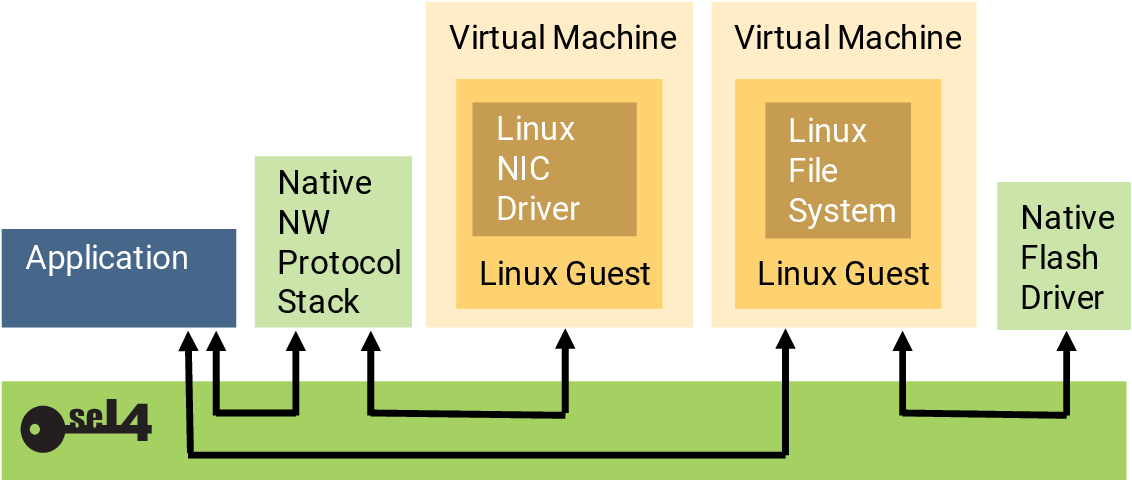
\includegraphics[width=\linewidth]{img/seL4Hypervisor.png}
  \caption{Virtualizzazione del SO Linux per l'integrazione dei servizi di networking e file system}
  \label{fig:Virtualizzazione}
\end{figure}
Queste due VM forniranno all'applicazione il servizio di networking e il file system per la gestione della memoria secondaria (hard disk, supporti rimovibili ecc.). Le comunicazioni tra le parti saranno gestite da un canale fornito dal microkernel, ma le due macchine virtuali non avranno modo di comunicare tra di loro. Come si vede in figura anche le comunicazioni tra le varie parti e l'applicazione sono ben delineate e precise, nessun'altra comunicazione al di fuori di quelle indicate dalle frecce è possibile.

\section{Capability}
Un concetto fondamentale in seL4 è quello di \textit{capability} che è definita formalmente come un riferimento ad oggetto. Possiamo definirla anche come un puntatore immutabile, cioè una capability farà sempre riferimento allo stesso oggetto.\\
SeL4 è un sistema capability-based (basato sulle capability) questo significa che l'unico modo per eseguire un'operazione è attraverso l'invocazione di una capability. Ad ognuna di esse, inoltre, sono associati dei diritti di accesso, quindi una capability è un incapsulamento di un riferimento ad oggetto con i diritti ad esso conferiti.
Per dare una definizione meno formale possiamo pensare alle capability come a delle chiavi di accesso estremamente specifiche riguardo quale entità può accedere ad una particolare risorsa del sistema. Per di più permettono di supportare il \textit{principle of least privilege}, principio del privilegio minimo chiamato anche \textit{principle of least authority} PoLA. Questo principio implica che ogni modulo deve avere accesso solo ed esclusivamente alle risorse strettamente necessarie al suo scopo.
In seL4 quindi i diritti dati ad un componente possono essere ristretti al minimo indispensabile per svolgere il loro lavoro, come richiesto dal PoLA, il che chiaramente è un grosso punto a favore per quanto riguarda la sicurezza.\\
Nei sistemi operativi più comuni tipo Windows o Linux l'accesso alle risorse è gestito dalle \textit{access-control list} (ACL). Quindi nel caso specifico di Linux, ad ogni file viene associato un set di bit che determinano quali operazioni (lettura, scrittura, esecuzione) possono essere eseguite su di esso dai vari utenti (proprietario, gruppo, altri). Tutto ciò implica che ogni file con lo stesso set di permessi è accessibile ad uno specifico utente. Se ci mettiamo nello scenario di voler avviare un programma, di cui non siamo sicuri della sua attendibilità, che abbia accesso ad uno e un solo file specifico questo non è possibile perchè come può accedere a quel file può accedere anche a tutti gli altri che hanno associati gli stessi permessi.\\
Con le capability questo scenario non si può presentare perchè il kernel consentirebbe un'operazione se e solo se chi richiede di eseguire l'operazione ha la "giusta capability" per eseguire l'operazione su quel file. 

\subsection{Proprietà delle capability}
Interposition: le capability hanno la proprietà di mettersi in mezzo (interpose) tra chi crea una capability e l'effettivo accesso ad una risorsa: se un utente dà una capability ad un oggetto esso non è in grado di sapere cosa effettivamente sia quell'oggetto, può chiaramente utilizzarlo senza però sapere che tipo di oggetto sia.\\
Delegation: le capability supportano la delegazione dei privilegi tra gli utenti: l'utente X ha un oggetto e vuole dare accesso ad esso anche all'utente Y; X può creare una nuova capability e darla ad Y senza conservare nessun riferimento all'utente X che l'ha creata, la nuova capability può anche avere meno diritti di accesso (esempio solo lettura invece di lettura e scrittura) e inoltre X in qualsiasi momento può revocare l'accesso ad Y distruggendo la capability.

\section{Hard Real-Time Systems}
Un \textit{Hard Real-Time System} è un sistema in cui il mancato rispetto di una scadenza può portare al fallimento dell'intero sistema. Un esempio molto comune e semplificato può essere l'autopilota di un'automobile. Un veicolo dotato di un software di guida autonoma richiede la presenza di un numero estremamente elevato di sensori esterni ed interni al veicolo e il computer di bordo deve leggere, elaborare e dare una risposta immediata ad ogni minimo cambiamento di un valore proveniente da questi sensori. Se ad un certo punto l'elaborazione di un dato richiede più del tempo dovuto, anche solo di qualche millisecondo, c'è il rischio che questo comporti una serie  di ritardi a catena che ad esempio portano al non rilevamento di un oggetto che si sta avvicinando al veicolo, oppure alla mancata correzione della traiettoria e quindi l'abbandono della carreggiata, con conseguenze anche catastrofiche.\\
seL4 ha alcune caratteristiche che lo rendono adatto in ambiti hard real-time.\\
Infatti, lo scheduling dei processi in seL4 è basato sulla priorità. Il kernel di sua iniziativa non cambierà mai la priorità di un processo, che è sempre decisa dall'utente.\\
Inoltre, quando seL4 esegue delle operazioni in modalità kernel queste sono esenti da interrupt. All'apparenza questo può sembrare catastrofico se non fosse per il fatto che le chiamate di sistema sono tutte brevi. Solo la revoca di una capability può richiedere tempi più lunghi ma in presenza di queste operazioni seL4 adotta una politica di divisione dell'esecuzione in sotto operazioni più brevi. In aggiunta ognuna di esse può essere annullata e poi ripresa da quel punto in poi, così da poter gestire degli eventuli interrupt in attesa.\\
Questi due punti appena elencati sono requisiti fondamentali per gli Hard Real-Time system: scheduling dei processi basato sulla priorità, che sia quindi facilmente analizzabile; latenza degli interrupt limitata, essendo gli interrupt disabilitati non ci sarà nessuna latenza dovuta al cambio di contesto per gestire subito l'interrupt e dato che le operazioni sono tutte brevi questo non risulta essere un problema.
Per seL4 è stata eseguita una worst-case execution time (WCET), questo vuol dire che è stato determinato un limite superiore di latenza di ogni system call nel caso peggiore, ciò implica anche il caso peggiore di latenza di un interrupt.

\subsection{Mixed-criticality systems}
Un mixed-criticality system (MCS) è un sistema fatto da più componenti che interagiscono tra di loro e che hanno differenti livelli di criticità. In questi sistemi è imperativo che il fallimento di un componente non influenzi gli altri componenti critici, e che questi siano quindi isolati e protetti dai componenti meno critici.\\
Un approccio classico per questo tipo di sistemi è isolare le criticità sia per quanto riguarda il tempo che lo spazio. Ciò è noto come \textit{strict time and space partitioning} (TSP). Ma questo implica dover assegnare staticamente l'area di memoria, il tempo di esecuzione e quindi lo scheduling, e per farlo si utilizzano dati misurati precedentemente nel caso pessimo. Essendo sistemi real-time, ogni operazione deve avere dei limiti di tempo, quindi un'operazione su cui è stato misurato un tempo di esecuzione di 5 millisecondi (sempre nel caso pessimo) deve avere questa durata, non 4ms nè tantomeno 6ms. Chiaramente determinando staticamente i tempi e gli spazi nel caso peggiore siamo sicuri che questi vengano rispettati. C'è da considerare però che non sempre si presentano dei casi pessimi dunque si ha uno scarso utilizzo delle risorse. Per di più la latenza di un interrupt nel caso pessimo può essere molto costosa.\\
seL4 supporta i mixed-criticality system. Per quanto riguarda l'isolamento, abbiamo già visto che le capability, in termini di spazio, intrinsecamente lo garantiscono. Resta quindi da esaminare il comportamento da un punto di vista temporale.\\
SeL4 normalmente utilizza due parametri per gestire lo scheduling dei processi: la priorità e la quantità di tempo. La \textit{priorità} determina l'ordine di esecuzione dei processi mentre la \textit{quantità di tempo} (time slice) determina quanto tempo il kernel lascerà in esecuzione un thread prima di fermarlo per selezionare un altro processo. Quest'ultimo verrà scelto tra i processi pronti in base alla priorità, con una politica round-robin tra i pari livelli di priorità. \\
La versione MCS di seL4 si comporta diversamente. L'accesso al processore viene controllato dalle capability, un componente può ottenere la CPU solo se ha una capability che glielo permette e il tempo di esecuzione è codificato in essa. Tale politica si chiama \textit{scheduling-context capabilities}. Lo scheduling-context contiene due attributi principali: 
\begin{enumerate}
	\item \textit{time budget} che sostituisce il time slice;
	\item \textit{time period} che determina invece quante volte un budget può essere usato per periodo, in questo modo viene evitato che un processo monopolizzi la CPU indipendentemente dalla sua priorità.
\end{enumerate}

\section{Sicurezza e performance}
Come già detto nelle prime righe di questo capitolo la famiglia dei microkernel L4 nasce per sopperire alle scarse performance dei suoi predecessori. Finora è stata fatta una descrizione del funzionamento generale di seL4 con particolare riguardo sulla sicurezza di questo sistema. Chi è dell'ambito sa già che spesso sicurezza e buone performance non vanno molto d'accordo. Garantire la sicurezza vuol dire attenersi a regole ben precise e controlli che spesso poi portano a rallentamenti e quindi vanno a influire sulle performance di un sistema. È dunque lecito domandarsi se questo microkernel sia performante oppure no.\\
Nonostante non fosse nelle prerogative dello sviluppo di seL4 questo, alla fine, si è rivelato il più performante dei microkernel della famiglia L4. Inoltre sono state fatte altre pubblicazioni indipendenti che mettono a confronto seL4 con altri microkernel per studiarne le performance, in particolare Fiasco.OC, Zicron \cite{skybridge} e CertiKOS \cite{CertiKOS}. Confrontando i costi dell'IPC si può vedere che seL4 ha un bel vantaggio anche di oltre un fattore due rispetto agli altri microkernel.